\documentclass[10pt]{article}

%\usepackage{times}

%\usepackage[margin=1.0in]{geometry}
%\usepackage{setspace}

\usepackage{enumerate}
\usepackage{graphicx}
\usepackage{float}

\usepackage{tipa}
\usepackage{qtree}
\usepackage{gb4e}

\usepackage{natbib}

\begin{document}
\title{This is a sample LaTeX document}
\author{You\\\texttt{netid@georgetown.edu}}
\date{\today}
\maketitle

\begin{abstract}
Lorem ipsum dolor sit amet, consectetur adipiscing elit. Ut vitae ultricies libero. Mauris placerat elementum elit ac ullamcorper. Curabitur porttitor cursus cursus. Nulla tincidunt nulla pellentesque erat volutpat sagittis. Morbi sem nunc, laoreet eu imperdiet et, accumsan viverra enim. Curabitur pellentesque erat et iaculis convallis. In eu elementum ligula, at pellentesque eros. Sed aliquam pellentesque nunc accumsan sollicitudin.
\end{abstract}

\section{Introduction}

%\doublespacing

Vivamus accumsan eget nisi \textit{consectetur consequat}. Phasellus vitae cursus urna. \textbf{Quisque rutrum}, ligula id volutpat porta, urna orci accumsan dui, ut blandit magna justo ullamcorper sem. Fusce rutrum, dui sit amet adipiscing imperdiet, libero urna lacinia nisl, et accumsan tellus arcu vitae justo. Ut tincidunt lectus eget faucibus convallis. Vestibulum ante ipsum primis in faucibus orci luctus et ultrices posuere cubilia Curae; Morbi tristique nibh quam, quis vulputate velit tempus vitae.

\subsection{Some more words}

\underline{In ligula felis}, dictum in lacus in, lacinia laoreet nunc. Vestibulum mollis arcu viverra tincidunt tincidunt. Proin pulvinar lacinia eros, eget pulvinar lectus tempor id. Lorem ipsum dolor sit amet, consectetur adipiscing elit. Nulla condimentum eu neque at egestas. Donec convallis, est eu consectetur posuere, nisl massa porttitor nunc, nec laoreet ante mauris quis lectus. Suspendisse elit enim, cursus sed scelerisque et, condimentum at justo. Proin sed fermentum dolor. Vivamus nec rutrum nisi. Vestibulum vehicula felis nec neque pretium blandit. Nullam dignissim ante nisl, at rutrum diam pellentesque faucibus. Nam in luctus sem. Vivamus ultricies tortor hendrerit egestas varius. Etiam mattis sagittis porttitor\footnote{Fusce volutpat diam vel cursus lacinia. Ut nec dolor sem. Nunc mi magna, dapibus quis est et, consequat ornare eros. Integer hendrerit molestie eros quis fringilla. Morbi vitae ornare leo, non viverra purus. Pellentesque eu mauris eget nunc mollis auctor et eget libero. In hac habitasse platea dictumst.}.


\section{Linguistics packages}

\subsection{tipa}

Duis iaculis justo in lacus convallis, non tristique urna mattis. Mauris porta nisl quis neque ornare, et dapibus dui consectetur. Phasellus sed tempor ante. Aliquam adipiscing ante arcu, id egestas augue imperdiet vitae.

``Would you meet me at the station at five?'':

\textipa{wUd ju mi:t mi \ae t D@ "steIS@n \ae t faIv}

\textipa{wUZu: mi:Pmi: \ae P D@ "steIS@n \ae:P faiv}


\subsection{gb4e}

Donec pellentesque, tellus a adipiscing tincidunt, urna justo viverra enim, ut scelerisque mauris ipsum porta turpis. Donec et leo ipsum. Sed laoreet lacus a augue ultricies vehicula. Aliquam faucibus pretium dolor, sollicitudin lobortis lectus sodales ut.

\begin{exe}
\ex \label{standardRel}
\underline{Standard German}
    \begin{xlist}
        \ex[]{\gll Der Mann, \textbf{der} aus M\"unchen kommt, gr\"u\ss t mich.\\
        the.\textsc{m.nom} man who.\textsc{m.nom} from Munich comes greets me\\
        \glt `The man who comes from Munich greets me.'}\label{standardRelMasc}
        
        \ex[]{\gll Die Frau, \textbf{die} zu Hause ist, liest gerne.\\
        the.\textsc{f.nom} woman who.\textsc{f.nom} at home is, reads gladly\\
        \glt `The woman who is at home reads gladly.'}\label{standardRelFem}
        
        \ex[*]{\gll Der Junge, \underline{\hspace{2em}} Max kennt, ist ein cooler Typ.\\
        the.\textsc{m.nom} boy {} Max knows is a cool dude\\
        \glt Intended: `The boy Max knows is a cool dude.'}\label{standardRelDPron}
        
        \ex[*]{\gll Das M\"adchen, das dass/was ein neues Auto gekauft hat, f\"ahrt zu schnell.\\
        the.\textsc{n.nom} girl who.\textsc{n.nom} that/what a new car bought has drives too fast\\
        \glt Intended: `The girl who bought a new car drives too fast.'}\label{standardRelComp}
    \end{xlist}
\end{exe}

\subsection{qtree}

Pellentesque vitae sollicitudin arcu, eget porttitor erat. Curabitur vel tristique sapien. Phasellus nec vehicula eros, vitae scelerisque elit. In hac habitasse platea dictumst. Praesent iaculis sodales augue, eget vulputate metus vestibulum vitae. In commodo egestas dui et bibendum. Nullam eu arcu mi. Morbi vitae consectetur magna, at scelerisque nibh. Reference to (\ref{tree}):

\begin{exe}
\ex
\Tree [.S This [.VP [.V is ] \qroof{a simple tree}.NP ] ]
\label{tree}
\end{exe}

\section{How about some lists?}

Curabitur eget enim vel erat facilisis ullamcorper vel eu leo. Mauris eu aliquet erat. Cum sociis natoque penatibus et magnis dis parturient montes, nascetur ridiculus mus. Ut fringilla tortor id est fermentum, vitae egestas augue fringilla. Maecenas et leo a ligula vulputate cursus. Donec gravida a magna quis pretium. Aliquam a ligula id lorem posuere gravida eget vitae sapien. In cursus est erat, at tristique magna bibendum eu. Donec egestas interdum bibendum. Sed neque velit, euismod non arcu ut, molestie tincidunt arcu. Integer mattis elit nibh, fermentum fringilla enim condimentum eget. Aliquam sed lectus suscipit, mattis ipsum nec, fringilla arcu:

%Here is a custom list style
\begin{enumerate}[I.]
\item{Vestibulum dignissim dolor eget ligula tincidunt feugiat.
\begin{enumerate}
\item{Integer in quam vulputate, egestas lectus nec, blandit turpis.\begin{enumerate}
\item{Fusce convallis quam at eros tristique, vel fringilla ante ullamcorper.}
\end{enumerate}}
\end{enumerate}}
\item{Donec sodales et risus non euismod.}
\item{Aenean mollis, nisl ut laoreet dignissim, mi erat fermentum tellus, vel viverra massa neque non purus.}
\item{Donec dictum, arcu ut varius bibendum, dolor ipsum interdum felis, tristique fermentum massa odio eu nunc.}
\item{Nulla at dictum ligula.}
\end{enumerate}

In a lorem sed tellus ornare congue. Integer orci massa, ornare eu enim vitae, porttitor euismod quam. Morbi fermentum ac quam a posuere. Donec venenatis condimentum lectus aliquet posuere. Sed et nulla vel purus ultrices vestibulum. Vestibulum felis enim, eleifend ut nulla vel, condimentum placerat ante. Vestibulum urna dui, varius ut libero sit amet, interdum viverra ante. Vestibulum posuere dignissim est. Cras condimentum vel orci at feugiat. Aliquam porttitor enim in justo fringilla faucibus:

\begin{itemize}
\item{Ut feugiat vitae arcu at iaculis.
\begin{itemize}
\item{Curabitur eget enim vel erat facilisis ullamcorper vel eu leo}
%Here is a custom bullet
\item[+]{Nullam egestas odio mi, nec sodales augue euismod bibendum.}
\end{itemize}}
\item{Mauris quis pharetra augue.}
\item{Praesent tristique iaculis felis, at semper magna auctor eget.}
\item{Suspendisse elementum augue nec commodo scelerisque.}
\item{Nulla accumsan lorem et est semper, id aliquet mi elementum.}
\end{itemize}

\section{Graphics}

\subsection{Plain graphics}

Maecenas consectetur purus vitae sagittis auctor. Pellentesque auctor sodales accumsan. Aliquam mattis risus sed ullamcorper rhoncus. Proin eu urna porttitor, tristique elit vel, fermentum ligula. Duis ipsum ligula, interdum nec nisi sit amet, sagittis aliquet ligula. Vivamus vestibulum, lorem eget pulvinar semper, quam lectus viverra augue, vitae mattis felis eros et nulla. Duis lacus est, porta tincidunt condimentum a, auctor id risus. Quisque ac erat vestibulum, ornare lorem quis, sagittis dui. Curabitur scelerisque ultrices metus. Quisque ornare diam at libero laoreet, et posuere magna vulputate. Fusce fringilla ullamcorper vestibulum. Praesent eget pellentesque elit. Suspendisse potenti. Donec interdum sapien non gravida feugiat. Nulla porta est sed justo varius, et suscipit dolor mollis. Interdum et malesuada fames ac ante ipsum primis in faucibus.

\begin{figure}[h]
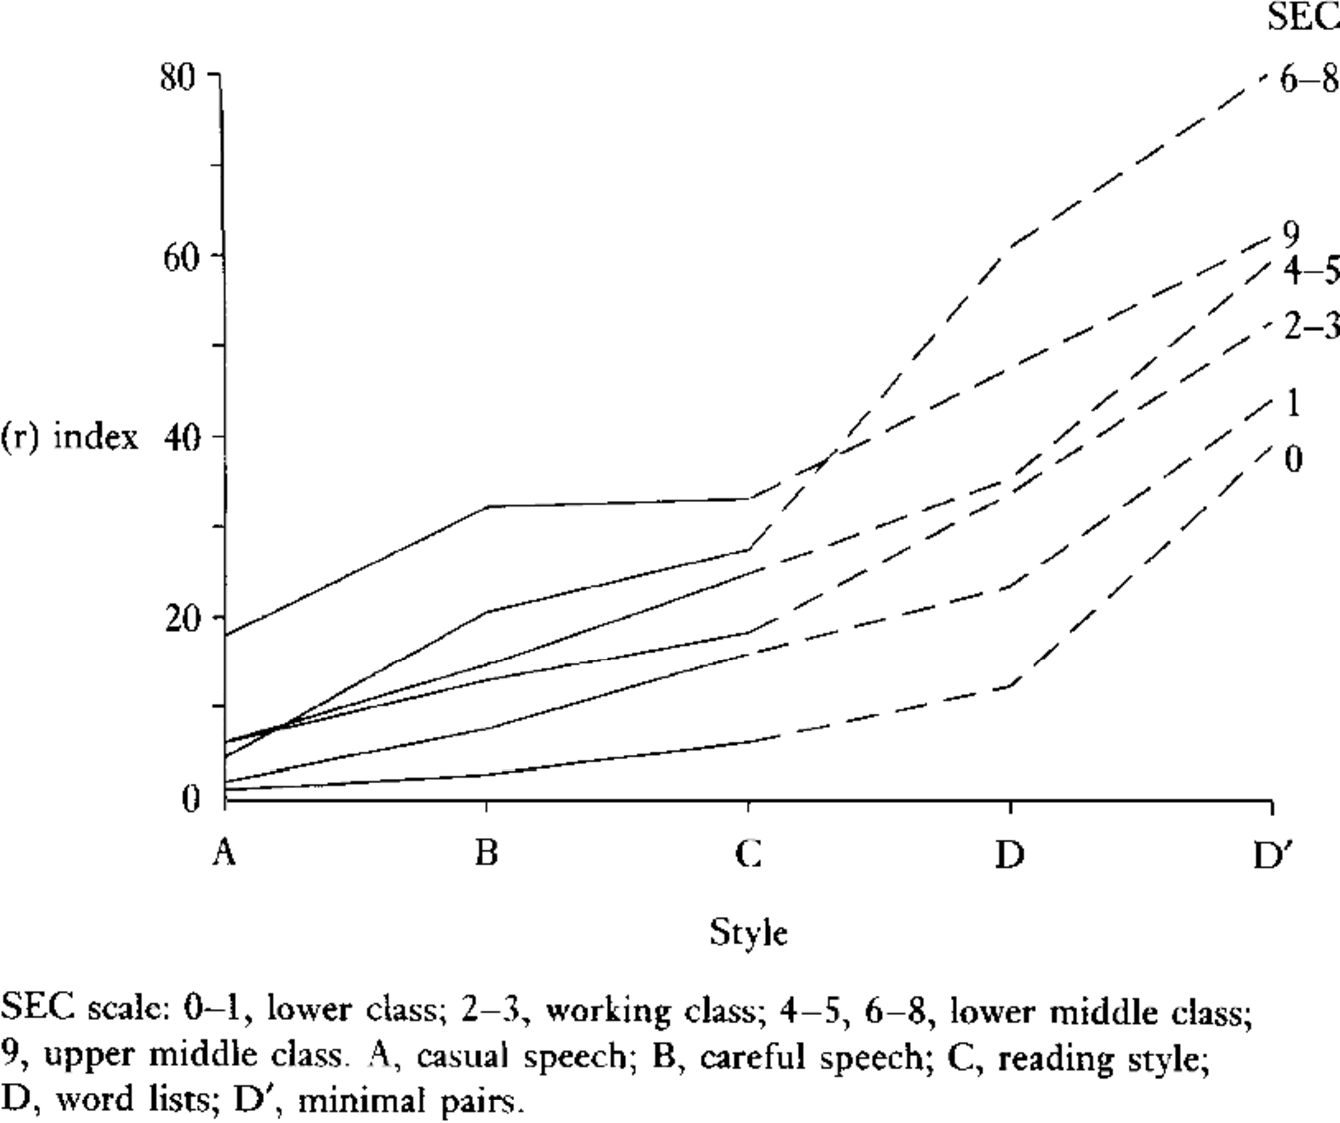
\includegraphics[width=0.95\textwidth]{LabovGraph.pdf}
\end{figure}

\subsection{More options}

Maecenas consectetur purus vitae sagittis auctor. Pellentesque auctor sodales accumsan. Aliquam mattis risus sed ullamcorper rhoncus. Proin eu urna porttitor, tristique elit vel, fermentum ligula. Duis ipsum ligula, interdum nec nisi sit amet, sagittis aliquet ligula. Vivamus vestibulum, lorem eget pulvinar semper, quam lectus viverra augue, vitae mattis felis eros et nulla. Duis lacus est, porta tincidunt condimentum a, auctor id risus. Quisque ac erat vestibulum, ornare lorem quis, sagittis dui. Curabitur scelerisque ultrices metus. Quisque ornare diam at libero laoreet, et posuere magna vulputate. Fusce fringilla ullamcorper vestibulum. Praesent eget pellentesque elit. Suspendisse potenti. Donec interdum sapien non gravida 
% Below is a reference
Figure~\ref{fig:simulation}. Nulla porta est sed justo varius, et suscipit dolor mollis. Interdum et malesuada fames ac ante ipsum primis in faucibus.

\begin{figure}[H]
\centering
    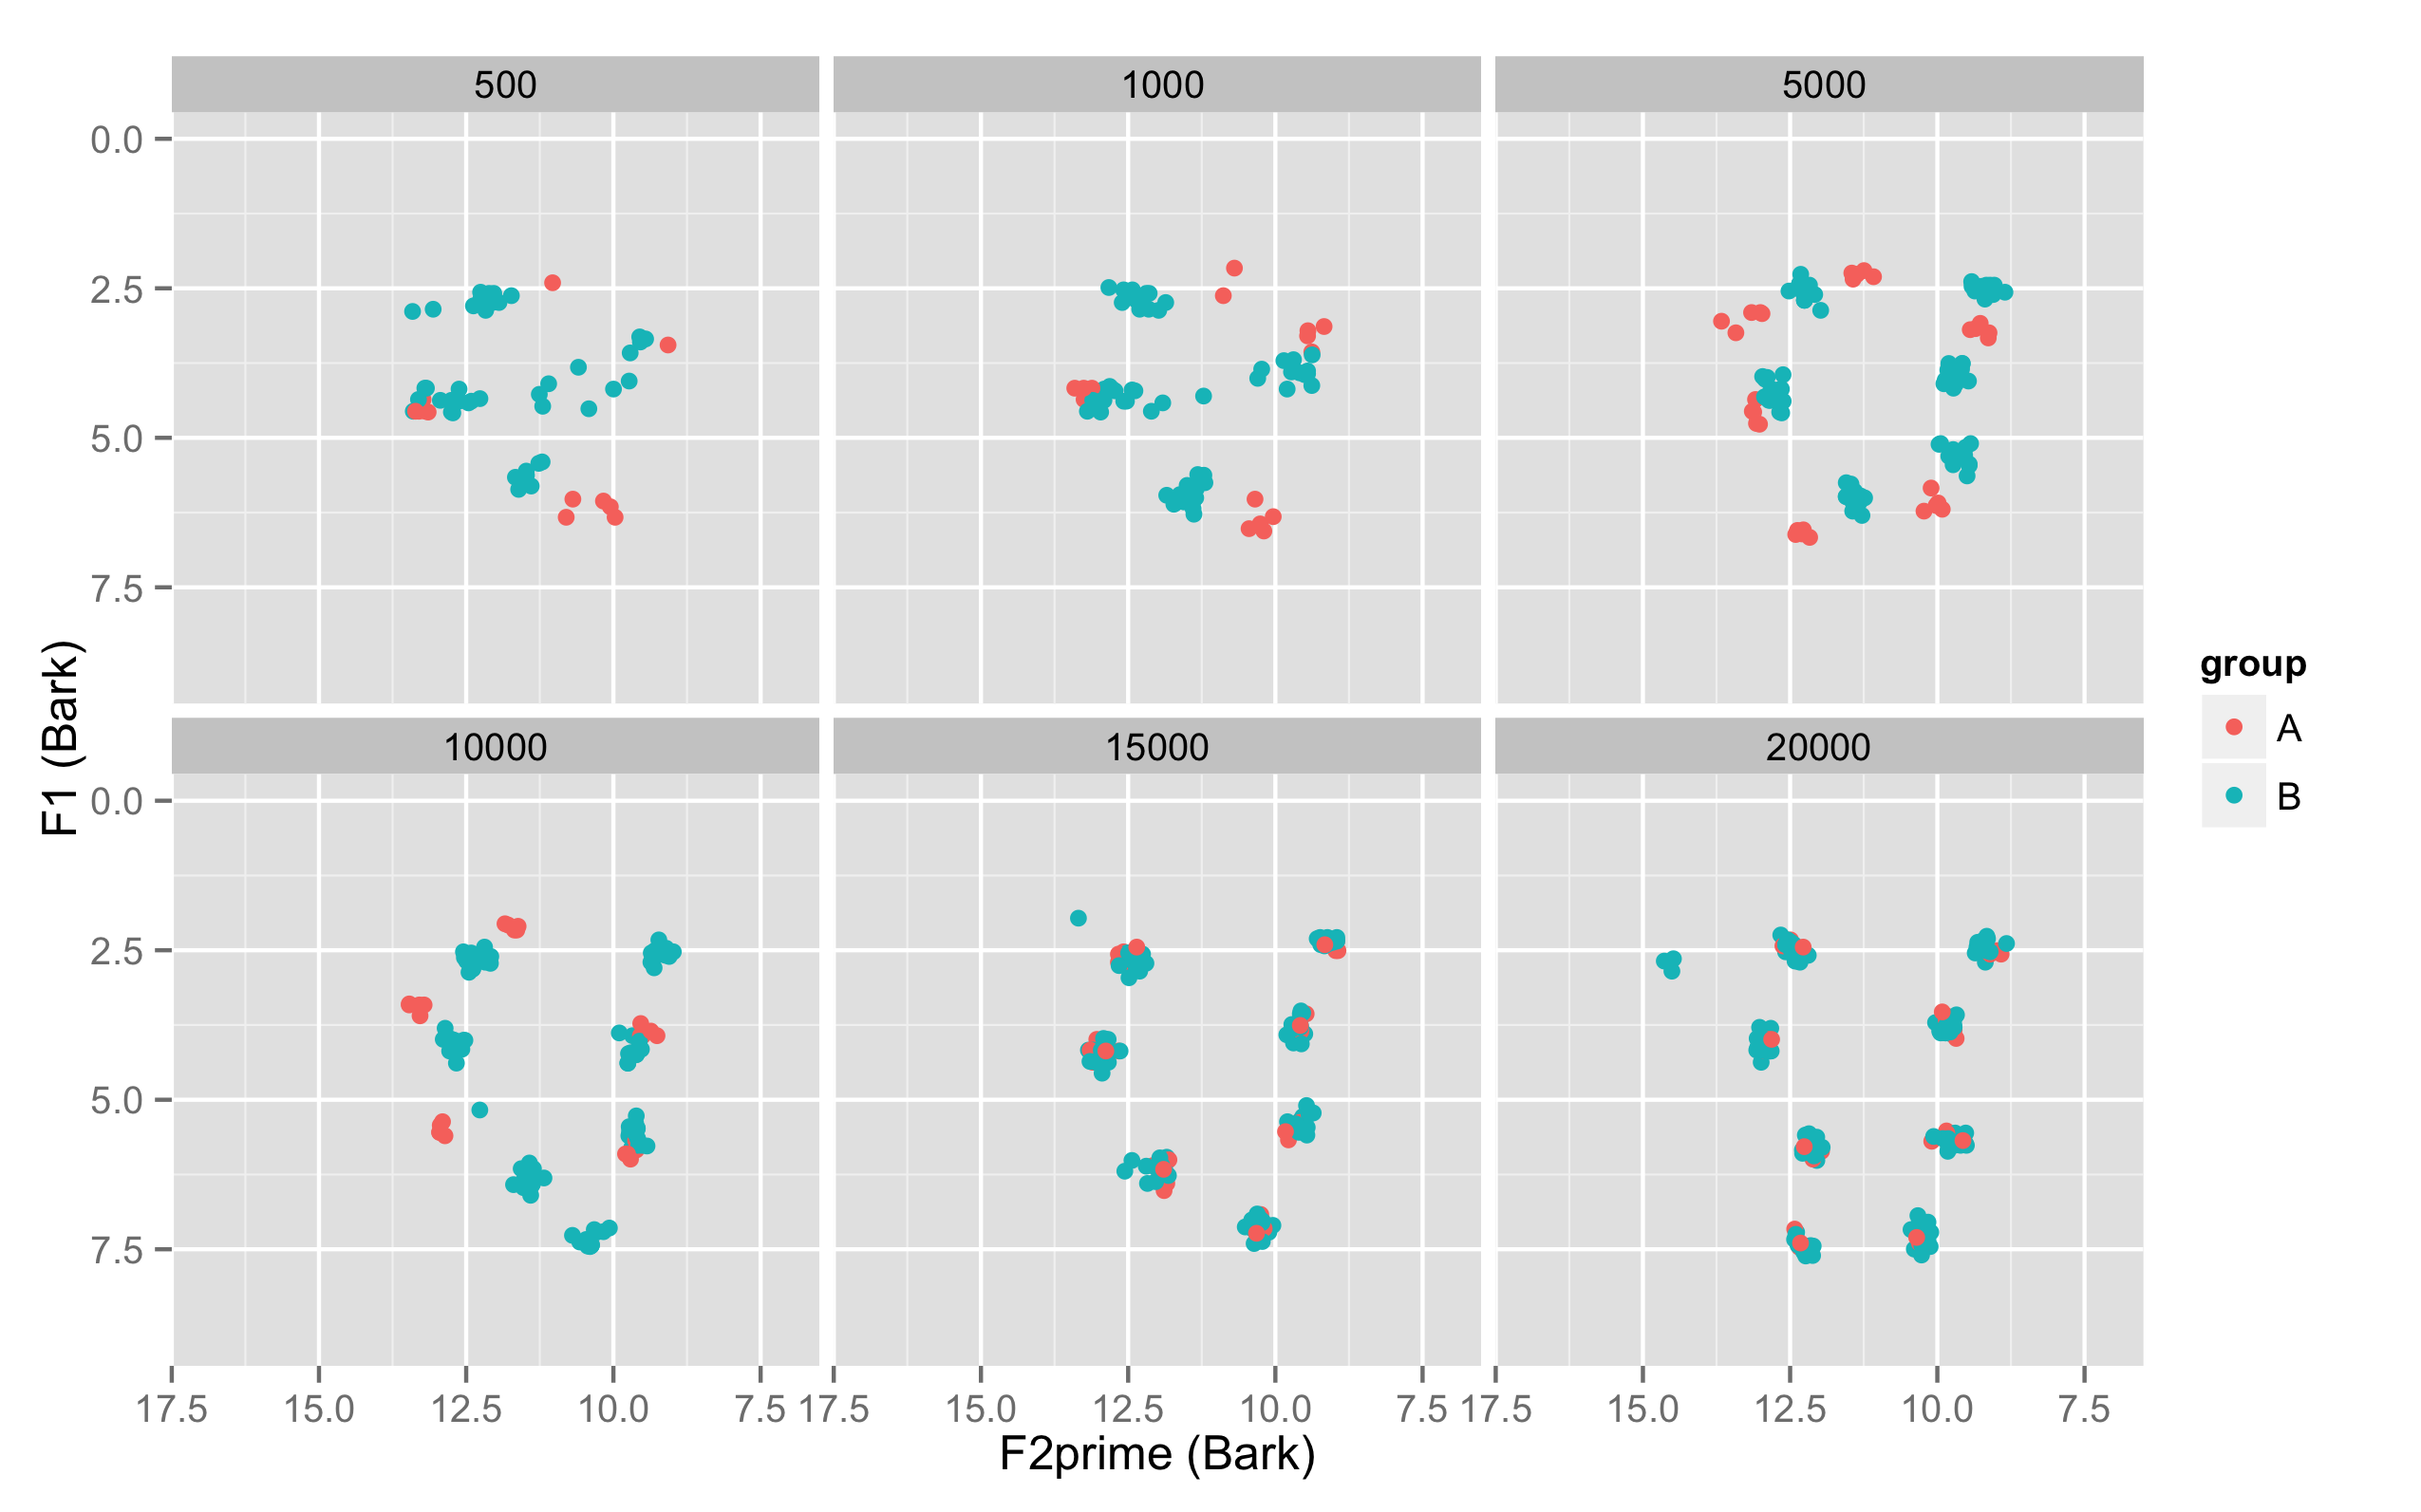
\includegraphics[width=0.95\textwidth]{VowelSpace.png}
  \caption{Some simulation results}
  \label{fig:simulation}
\end{figure}


\end{document}